\section{Contesto e Finalità}
Per comprendere nella sua complessità il progetto elaborato in questa tesi è necessario tenere conto, prima di tutto, del contesto in cui viene sviluppato e delle finalità implicite ed esplicite che si vogliono raggiungere.
In questo caso si tratta di descrivere lo sviluppo di un applicativo mobile fortemente legato ai sistemi di marketing e alle nuove strategie di business di aziende leader all'interno dei propri mercati, in molti casi saturi o fortemente instabili, scossi dalle innovazioni tecnologiche di questi decenni.

Oltre alle ingerenze esterne sul progetto, come il cambiamento repentino delle tecnologie o la presenza di eventuali competitor, deve essere valutata la posizione del singolo componente all'interno dello sviluppo dell'interno progetto, la quale va tenuta in forte considerazione specialmente durante la prima fase di sviluppo in cui si determinano le prime linee guida da seguire durante tutto il lavoro.

Questo elaborato rientra nel concetto di \textit{Application Economy}, che descrive perfettamente il trend degli ultimi anni: il cambiamento dei metodi con cui le masse ottengono informazioni e si lasciano influenzare hanno portato ad un sostanziale sconvolgimento del sistema di marketing e delle strategie commerciali anche di aziende multinazionali. 
Proprio in questo contesto è necessario inquadrare le motivazioni che hanno portato l'azienda Carpigiani a dare vita all'ecosistema MyGelato, di cui questa tesi sviluppa solo una componente, così da realizzare quanto progetti di questo tipo siano fondamentali in questo momento storico.
Si tratta di uno studio con finalità esplicite in ambito pubblicitario e con finalità implicite legate, invece, all'ambito commerciale e produttivo dell'azienda.


\subsection{Application Economy}
  
\begin{figure}[h!]
  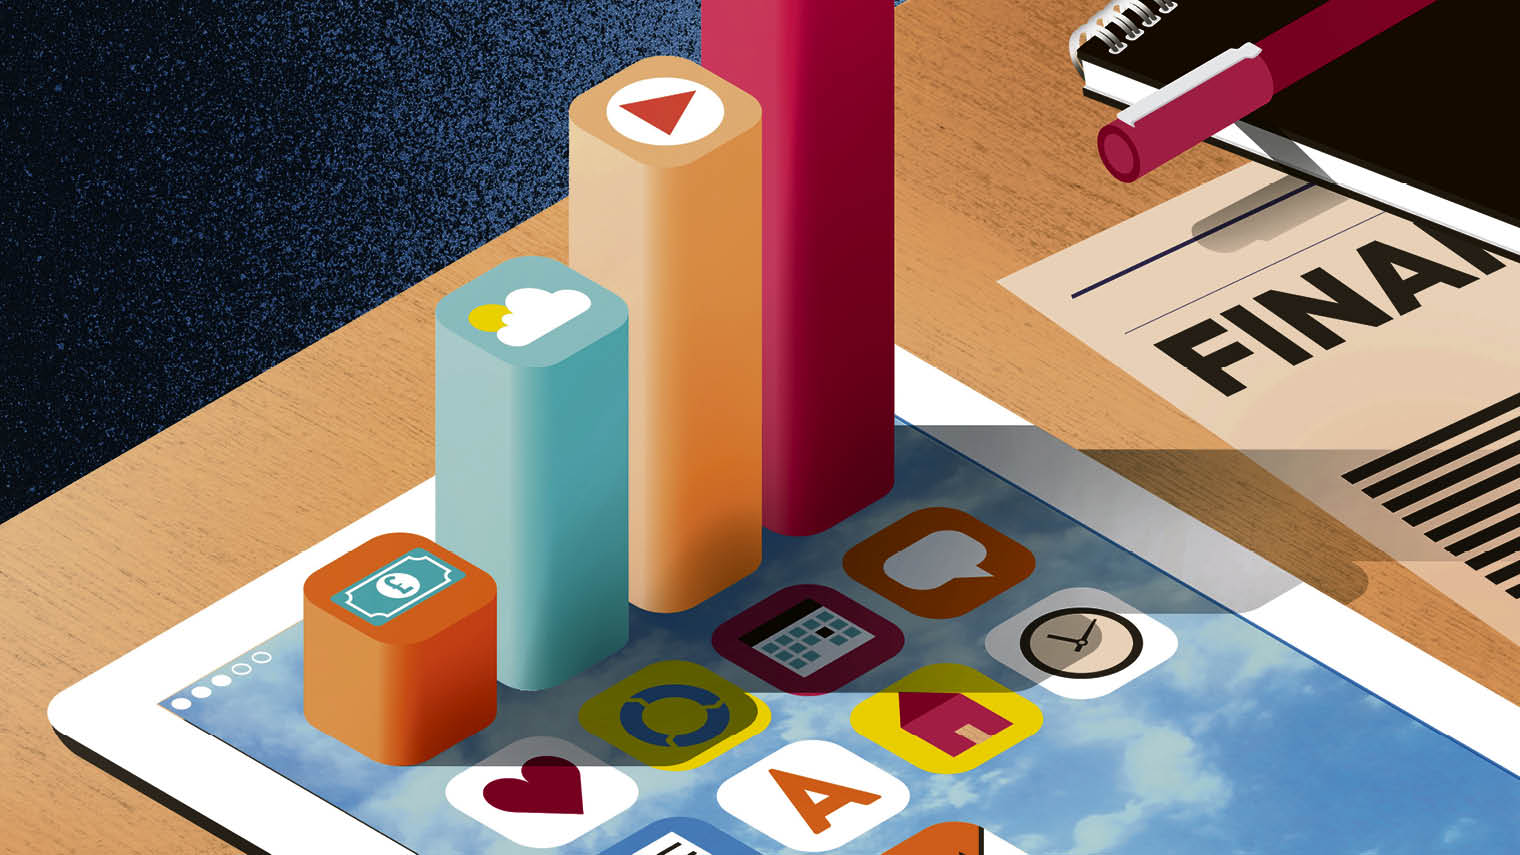
\includegraphics[width=\linewidth]{images/The-App-Economy.jpg}
  \caption{Applications Economy}
  \label{fig:appEconomy1}
\end{figure}
  
Non vi è forse modo di descrivere la società attuale e questo periodo storico senza valutare l'importanza dello sviluppo tecnologico che ci ha portato in quella che viene definita l'\textit{Era dell'Informazione}.
La rivoluzione tecnologica che sta avvenendo in questi anni, specialmente a partire dagli anni Novanta, ha portato la connessione globale a internet ad assumere un ruolo essenziale in ogni aspetto della società moderna e della nostra vita.

È cambiato drasticamente il modo con cui le persone accedono alle informazioni, che siano queste di tipo personale o di tipo commerciale.
Allo stesso modo si sono dovute adeguare le strategie di tutte quelle aziende che hanno visto cambiare in maniera drastica il proprio mercato, invaso molte volte da tecnologie sempre diversificate e innovative.

Secondo il giornalista Paul Mason, è stata la dottrina economica degli ultimi decenni della nostra epoca che da una parte ha avuto il merito di promuovere la più grande ondata di sviluppo economico che il mondo abbia mai visto, ma dall’altra ha portato a mercati incontrollati e a vorticosi cambiamenti sociali innescati dalla tecnologia.
Si sono diffusi, infatti, concetti come i progetti open-source, la sharing economy e le licenze creative commons che hanno messo in crisi le fondamenta del capitalismo odierno.
Questo fenomeno unito alla saturazione di molti mercati ha portando tante aziende a dover rivedere la propria business strategy obbligandole a dirigere i propri investimenti sulla diversificazione e sulle nuove strategie di vendita. \autocite{POSTCAPITALISMO}

Si sono evoluti tutti i meccanismi di commercializzazione di un prodotto: primi su tutti sono diventati di fondamentale importanza i concetti di e-commerce e marketing digitale, fortemente spinti dalle tecnologie e dalla nuova possibilità di accedere a una risorsa comune (Internet) da parte della maggior parte della persone anche di cultura, età e ambienti sociali diversi.
L'utente medio, per esempio, viene ormai maggiormente raggiunto e conivolto tramite email pubblicitarie o advertising online rispetto a meccanismi ormai meno incisivi di marketing non digitale.

Legato alla diffusione sempre crescente di smartphone, che sono diventati molte volte l'accesso principale degl utenti a internet, nasce quindi l'\textit{Application Economy}: lo sviluppo e l'utilizzo di applicazioni mobile per raggiungere i consumatori.
Tramite un applicativo mobile è quindi possibile svolgere una serie di azioni online con semplicità e in mobilità; potendo confidare, nella maggior parte dei casi, in un'alta sicurezza della propria connessione e nello scambio dei dati.

Se questa strategia può essere applicata, per esempio, in ambito marketing per pubblicizzare un proprio prodotto e fidelizzare il consumatore alla propria azienda, è forse più incisivo come l'e-commerce abbia ormai soppiantato la commercializzazione tradizionale in molti ambiti, specialmente tramite applicativi mobile (una statistica del BI Intelligence riporta che entro il 2020 il commercio mobile supererà il 45\% degli acquisti online complessivi).
L'abbattimento dei costi di un rivenditore non fisico e la nascita di servizi di pagamento online come PayPal hanno portato questa rivoluzione in ogni ambito commerciale permettendo, inoltre, all'utente di pagare direttamente tramite sistemi bancari in sicurezza e con semplicità.

Tutti questi concetti sono ormai più che affermati in ambiti come la vendita di prodotti di abbigliamento o tecnologici ma l'azienda Carpigiani ha scelto di portare questi nuovi meccanismi anche all'interno del proprio campo, quello delle Gelaterie, in modo innovativo grazie al progetto MyGelato.

\subsection{Ecosistema MyGelato}

L'ecosistema MyGelato si pone all'interno contesto descritto all'interno del capitolo precedente, a unire le strategie di marketing dell'azienda produttrice Carpigiani e delle singole gelaterie convenzionate; insieme alla possibilità di comprare, regalare e utilizzare online dei coupon che permettono l'acquisto di gelati.

È un progetto di piattaforma web e mobile che si rivolge al pubblico dei gelatieri e dei consumatori di gelato. Gli obiettivi commerciali sono diversi, primi tra i quali quello di incentivare la compravendita di gelati tramite il sistema di coupon digitali e quello di promuovere il consumo di gelato tramite offerte, fornendo anche ai gelatieri un sistema semplice ed efficace per pubblicizzare il proprio negozio.

Attraverso l'applicativo, l'utente può informarsi sulle gelaterie presenti in zona verificando anche quali facciano parte del circuito MyGelato: insieme delle gelaterie convenzionate alla vendita e alla validazione dei coupon online.
È possibile selezionare ogni gelateria così da avere alcune informazioni utili, come indirizzo e numero di telefono, salvarle nei preferiti e verificare se vi sono promozioni attive.
Nel momento in cui l'utente aggiunge ai preferiti una gelateria, verrà informato tramite notifica push di eventuali nuove promozioni attive e sarà notificato anche nel caso in cui si avvicini a una gelateria di proprio interesse.
Queste strategie sono ovviamente di carattere pubblicitario e permettono anche a gelaterie minori, facenti però parte del circuito, di essere pubblicizzate agli utenti che utilizzano la piattaforma.

Questo sistema permette all'azienda Carpigiani di avere un controllo maggiore su un sistema centralizzato di advertasing per le gelaterie di cui è principale fornitore, ottenendo quindi la possibilità di intervenire su realtà locali standardizzandone alcuni meccanismi.

Seconda feature fondamentale dell'applicazione, che riguarda in questo caso solo gli utenti iscritti al sistema, è la possibilità di comprare online dei coupon digitali che permetto l'acquisto, tramite validazione, di un gelato presso una determinata gelateria.
Questi coupon sono visualizzabili in ogni momento e possono essere regalati anche ad altri utenti tramite un semplice metodo di condivisione/riscatto che permette al destinatario di usufruire dell'oggetto comprato.
Ogni gelateria che supporta questo sistema sarà provvista della stessa applicazione con un account specifico per il gelatiere che permetterà di validare i coupon utilizzati e ricevere il proprio compenso tramite il sistema di pagamento online.

Questo sistema di e-commerce sposta la vendita di un prodotto molto semplice come i gelati, online; È infatti possibile comprarli tramite carta di credito e l'azienda Carpigiani, nel frattempo, ottiene così informazioni legate alle realtà locali a cui altrimenti non avrebbe accesso.
Questo sistema, per quanto diffuso in altri mercati come il reseller online di oggettistica è fortemente innovativo in questo campo e rende l'ecosistema MyGelato uno dei primi nel suo settore.

\newpage